\documentclass[11pt,oneside,a4paper]{book}
\usepackage[a4paper]{geometry}
\usepackage[utf8]{inputenc}
\usepackage[T1]{fontenc}
\usepackage[english]{babel}
\usepackage{datetime}
\usepackage{epigraph}
\usepackage{textcomp}
\usepackage{amsmath}
%\usepackage{amsfonts}
%\usepackage{amssymb}
%\usepackage[dvips]{graphicx}
\usepackage{lastpage}
%\usepackage{pst-node}
%\usepackage{bigdelim}
%\usepackage{multirow}
\usepackage{url}
\usepackage[printonlyused]{acronym}
\usepackage{algpseudocode}
\usepackage{algorithm}
\usepackage{tikz}
%\usepackage{tikz-timing}
\usepackage{bytefield}
\usepackage{srclist}
\usetikzlibrary{calc,trees,positioning,arrows,chains,shapes.geometric,%
    decorations.pathreplacing,decorations.pathmorphing,shapes,%
    matrix,shapes.symbols,fit}

\tikzset{
>=stealth',
  punktchain/.style={
    rectangle,
    rounded corners,
    % fill=black!10,
    draw=black, very thick,
    text width=10em,
    minimum height=3em,
    text centered,
    on chain},
  line/.style={draw, thick, <-},
  element/.style={
    tape,
    top color=white,
    bottom color=blue!50!black!60!,
    minimum width=8em,
    draw=blue!40!black!90, very thick,
    text width=10em,
    minimum height=3.5em,
    text centered,
    on chain},
  every join/.style={->, thick,shorten >=1pt},
  decoration={brace},
  tuborg/.style={decorate},
  tubnode/.style={midway, right=2pt},
}

\pgfdeclarelayer{background}
\pgfsetlayers{background,main}


\title{%
  Zeke\\
  A kernel for ARM processors
}
\author{%
  Olli Vanhoja\\
  \texttt{olli.vanhoja@cs.helsinki.fi}
}
\date{%
Generated: \today
}

\pagestyle{plain}
\begin{document}
  \maketitle
  \tableofcontents

  \part{Introduction}

Zeke is a portable operating system mostly targetted for ARM
processors.\footnote{Zeke is portable to at least in a sense of portability
    between different ARM cores and architectures.}
Zero Kernel, as it was originally known, is a tiny kernel implementation that
was originally targeted for ARM Corex-M microcontrollers. The reason to start
this project was that most of RTOSes available at the time for M0 feeled less
or more bloated for very simple applications. Secondly I found architectures
based on ARMv6-M to be quite challenging and interesting platforms for
RTOS/kernel development, especially when ARMv6-M is compared to ARMv7-M used
in M4 core or any Cortex-A cores using real ARM architectures.

One of the original goals of Zero Kernel was to make it CMSIS-RTOS compliant
where possible, as some concepts of Zeke were not actually CMSIS compliant
from the begining. However the scope of the project shifted pretty early and
the kernel is no longer CMSIS compatible at any level. Currently Zeke is
moving towards POSIX-like system and its user space is taking a Unix-like
shape. Nowadays Zeke is a bit bloatty when compared to the original standard
of a bloated OS but I claim Zeke is still quite tightly integrated system,
compared to any other Unix-like OS implementation.

Figure \ref{figure:zeke} illustrates architectural layers of the operating
system. Scope of Zeke project is to implement a portable
Unix-like\footnote{The project is aiming to implement the core set of kernel
    features specified in \ac{POSIX} standard.} operating system from
scratch\footnote{At least almost from scratch, some functionality is derived
from BSD kernels as well as some libraries are taken from other sources.} that
is optimized for ARM architectures and is free of legacy.

In addition to portability another long standing goal has been configurability
and adjustable footprint of the kernel binary as well as the whole OS image.
This is achieved by modular kernel architecture and static compile time
configuration. Like for example \ac{HAL} selection is already almost fully
locked at compilation time.

\begin{figure}
  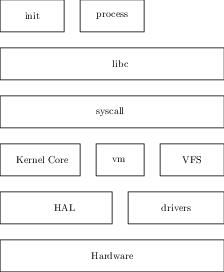
\includegraphics[width=10cm]{pics/zeke}
  \centering
  \caption{Zeke: a Portable Operating System.}
  \label{figure:zeke}
\end{figure}

\section*{List of Abbreviations and Meanings}

\begin{acronym}[UniversalSpacer]
\acro{POSIX}[POSIX]{Portable Operating System Interface for uniX\acroextra{ is a
  family of standards specifying a standard set of features for compatibility
  between operating systems.}}
\acro{HAL}[HAL]{Hardware Abstraction Layer\acroextra{.}}

\acro{inode}[inode]{\acroextra{inode is the file index node in Unix-style file
  systems that is used to represent a file file system object.}}
\acro{lfn}[LFN]{Long File Name\acroextra{.}}
\acro{mbr}[MBR]{Master Boot Record\acroextra{.}}
\acro{ramfs}[ramfs]{RAM file system\acroextra{.}}
\acro{sfn}[SFN]{Short File Name\acroextra{.}}
\acro{vfs}[VFS]{Virtual File System\acroextra{.}}
\acro{vnode}[vnode]{\acroextra{vnode is like inode but it's used as an
  abstraction level for compatibility between different file systems in Zeke.
  Particularly it's used at VFS level.}}

\acro{bio}[bio]{IO Buffer Cache\acroextra{.}}
\acro{dynmem}[dynmem]{(dynamic memory)\acroextra{ is the block memory allocator
  system in Zeke, allocating in 1 MB blocks.}}
\acro{vralloc}[VRAlloc]{Virtual Region Allocator\acroextra{.}}

\acro{MIB}[MIB]{Management Information Base\acroextra{ tree.}}

\acro{ipc}[IPC]{Inter-Process Communication\acroextra{.}}
\acro{shmem}[shmem]{Shared Memory\acroextra{.}}
\acro{rcu}[RCU]{Read-Copy-Update\acroextra{.}}

\acro{elf}[ELF]{Executable and Linkable
  \acroextra{ or Extensible Linking Format.}}

\acro{PUnit}[PUnit]{a portable unit testing framework for C\acroextra{.}}
\acro{GCC}[GCC]{GNU Compiler Collection\acroextra{.}}
\acro{GLIBC}[GLIBC]{The GNU C Library\acroextra{.}}
\acro{CPU}[CPU]{Central Processing Unit\acroextra{ is, generally speaking, the
  main processor of some computer or embedded system.}}

\acro{DMA}[DMA]{Direct Memory Access\acroextra{ is a feature that allows
 hardware subsystems to commit memory transactions without \acsu{CPU}'s
 intervention.}}
\acro{PC}[PC]{Program Counter\acroextra{ register .}}
\end{acronym}


  \part{Memory Management}

\chapter{An Overview to Memory Management in Zeke}

In this chapter we will briefly introduce the architectural layout of memory
management in Zeke. Zeke as well as most of major operating systems divides
its memory management and mapping to several layers to hide away any hardware
differences and obscurities. In Zeke these layers are \ac{MMU} \acs{HAL} that
abstracts the hardware, \verb+dynmem+ handling the dynamic allocation of
contiguous blocks of memory and \verb+kmalloc+ that allocates memory for the
kernel itself, and probably most importantly \verb+vralloc/buf/bio+ subsystem
that's handling all allocations for processes and IO buffers. Relations between
different kernel subsystems using and implementing memory management are shown
in figure \ref{figure:vmsubsys}.

\begin{figure}
\begin{verbatim}
U                      +---------------+
S                      |    malloc     |
R                      +---------------+
------------------------------ | -----------
K   +---------------+  +---------------+
E   |    kmalloc    |  |     proc      |
R   +---------------+  +---------------+
N           |     /\    |      |
E           |     |    \/      |
L  +-----+  |  +---------+   +----+
   | bio |--|--| vralloc |---| vm |
   +-----+  |  +---------+   +----+
            |     |            |
           \/    \/            \/
    +---------------+     +----------+
    |    dynmem     |-----| ptmapper |
    +---------------+     +----------+
            |                  |
           \/                  |
    +---------------+          |
    |    mmu HAL    |<----------
    +---------------+
            |
    +-----------------------+
    | CPU specific MMU code |
    +-----------------------+
----------- | ------------------------------
H   +-------------------+
W   | MMU & coProcessor |
    +-------------------+
\end{verbatim}
\caption{Memory management related subsystems and main users of the subsystems
         in Zeke.}
\label{figure:vmsubsys}
\end{figure}

\begin{itemize}
  \item \verb+kmalloc+  - is a kernel level memory allocation service, used
                        solely for memory allocations in kernel space.
  \item \verb+vralloc+  - VRAlloc is a memory allocator targeted to allocate
                        blocks of memory that will be mapped in virtual
                        address space of a processes, but it's widely used
                        as a generic allocator for medium size allocations,
                        it returns a \verb+buf+ structs that are used to
                        describe the allocation and its state.
  \item \verb+bio+      - is a IO buffer system, mostly compatible with the
                        corresponding interface in BSD kernels,
                        utilizing vralloc and buf system.
  \item \verb+dynmem+   - is a dynamic memory allocation system that allocates
                        \& frees contiguous blocks of physical memory (1 MB).
  \item \verb+ptmapper+ - owns all statically allocated page tables
                        (particularly the master page table) and regions,
                        and it is also used to allocate new page tables from
                        the page table region.
  \item \verb+vm+       - vm runs various checks on virtual memory access,
                        copies data between user land, kernel space and
                        allocates and maps memory for processes, and wraps
                        memory mapping operations for proc and \acs{bio}.
  \item mmu HAL -       is an interface to access MMU, provided by \verb+mmu.h+
                        and \verb+mmu.c+.
  \item CPU specific MMU code is the module responsible of configuring the
        physical MMU layer and implementing the HW interface provided by
        \verb+mmu.h+
\end{itemize}

\begin{table}
\caption{The memory map of Zeke running on BCM2835.}
\label{table:bcm_memmap}
\begin{tabular}{l|c|l}
Address                     &   & Description                   \\
\hline
\textbf{Interrupt Vectors}  &   &                               \\
0x0 - 0xff                  &   & Not used by Zeke              \\
0x100  - 0x4000             & L & Typical placement of ATAGs    \\
\textbf{Priv Stacks}        &   &                               \\
0x1000 - 0x2fff             & Z & Supervisor (SWI/SVC) stack    \\
0x3000 - 0x4fff             & Z & Abort stack                   \\
0x5000 - 0x5fff             & Z & IRQ stack                     \\
0x6000 - 0x6fff             & Z & Undef stack                   \\
0x7000 - 0x7fff             & Z & System stack                  \\
0x8000 - 0x3fffff           & Z & Kernel area (boot address)    \\
0x00400000-                 & Z & Page Table                    \\
0x007FFFFF                  &   & Area                          \\
0x00800000                  & Z & Dynmem                        \\
0x00FFFFFF                  &   & Area                          \\
-                           &   &                               \\
\textbf{Peripherals}        &   &                               \\
0x20000000 -                &   &                               \\
\textit{Interrupts}         &   &                               \\
0x2000b200                  & B & IRQ basic pending             \\
0x2000b204                  & B & IRQ pending 1                 \\
0x2000b20c                  & B & IRQ pending 2                 \\
0x2000b210                  & B & Enable IRQs 1                 \\
0x2000b214                  & B & Enable IRQs 2                 \\
0x2000b218                  & B & Enable Basic IRQs             \\
0x2000b21c                  & B & Disable IRQs 1                \\
0x2000b220                  & B & Disable IRQs 2                \\
0x2000b224                  & B & Disable Basic IRQs            \\
- 0x20FFFFFF                & B & Peripherals
\end{tabular}

\begin{tabular}{l|l}
\multicolumn{2}{c}{} \\
\multicolumn{2}{c}{Legends} \\
\hline
Z & Zeke specific \\
L & Linux bootloader specific \\
B & BCM2835 firmware specific mappings
\end{tabular}
\end{table}

\acrodef{MMU}[MMU]{Memory Management Unit}

\chapter{\acl{MMU} \acs{HAL}}

% - MMU in general
% - ARM MMU
% -- L1 & L2 page tables on ARM
% -- master page table and page table in Zeke
% -- regions in zeke


% The page table abstraction system in the kernel is relatively
% light but it still allows things that are not usually
% directly achievable with a plain harware implementation, eg. variable sized
% page tables.

\textbf{ARM11 note:} Only 4 kB pages are used with L2 page tables thus
XN (Execute-Never) bit is always usable also for L2 pages.

\subsection{Domains}

See \verb+MMU_DOM_xxx+ definitions.


\chapter{dynmem}

Dynmem is a memory block allocator that always allocates memory in
$1 \:\textrm{MB}$ blocks. See fig. \ref{figure:dynmem_blocks}.
Dynmem allocates its blocks as $1 \:\textrm{MB}$ sections from the L1 kernel
master page table and always returns physically contiguous memory regions. If
dynmem is passed for a thread it can be mapped either as a section entry or
via L2 page table, though this is normally not done as the vm interface is
used instead, though this is normally not done as the vm interface is
used instead.

\begin{figure}
  \input{pics/dynmem_blocks}
  \centering
  \caption{An example of reserved regions in dynmem.}
  \label{figure:dynmem_blocks}
\end{figure}

\chapter{kmalloc}

The current implementation of a generic kernel memory allocator is largely
based on a tutorial written by Marwan Burrelle\cite{Burelle:malloc}.

\section{The implementation}

The current kernel memory allocator implementation is somewhat naive and
exploits some very simple techniques like the first fit algorithm for allocating
memory.

The idea of the first fit algorithm is to find a first large enough free block
of memory from an already allocated region of memory. This is done by traversing
the list of memory blocks and looking for a sufficiently large block. This is
of course quite sub-optimal and better solutions has to be considered in the
future. When a large enough block is found it's split in two halves so that the
left one corresponds to requested size and the right block is left free. All data
blocks are aligned to 4 byte access.

Fragmentation of memory blocks is kept minimal by immediately merging newly freed
block with neighboring blocks. This approach will keep all free blocks between
reserved blocks contiguous but it doesn't work if there is lot of allocations of
different sizes that are freed independently. Therefore the current implementation
will definitely suffer some fragmentation over time.

When kmalloc is out of (large enough) memory blocks it will expand its memory
space by allocating a new block of memory from dynmem. Allocation is commited in
1 MB blocks (naturally) and always rounded to the next 1 MB.

\begin{figure}
\begin{bytefield}{16}
    \wordbox{1}{Descriptor} \\
    \wordbox[lrt]{1}{Free} \\
    \skippedwords \\
    \wordbox[lrb]{1}{} \\
    \wordbox{1}{Descriptor} \\
    \wordbox[lrt]{2}{Data} \\
    \skippedwords
\end{bytefield}
\caption{Kmalloc blocks.}
\label{figure:kmalloc_blocks}
\end{figure}

Descriptor structs are used to store the size of the data block, reference counters,
and pointers to neighbouring block descriptors.


\section{Suggestions for further development}

\subsection{Memory allocation algorithms}

The current implementation of kmalloc relies on first-fit algorithm and variable
sized blocks, that are processed as a linked list, which is obviously inefficient.

One achievable improvement could be adding a second data structure that would
maintain information about free memory blocks that could be used to store the
most common object sizes. This data structure could be also used to implement
something like best-fit instead of first-fit and possibly with even smaller
time complexity than the current implementation.

\begin{eqnarray}
\mathrm{proposed\_size} &=& \mathrm{req\_size}
  + \frac{\mathrm{curr\_size}}{\mathrm{req\_size}} \mathrm{o\_fact}
  + \frac{\mathrm{curr\_size}}{o\_div}.
\end{eqnarray}

\begin{algorithm}
  \caption{krealloc over commit}
  \label{algo:realloc_oc}
  \begin{algorithmic}
      \If{$\mathrm{req\_size} > \mathrm{proposed\_size}$}
        \State $\mathrm{new\_size} \gets \mathrm{req\_size}$
      \Else
        \If{$\mathrm{limit}_{min} < 4 \frac{proposed\_size}{req\_size} < \mathrm{limit}_{max}$}
          \State $\mathrm{new\_size} \gets \mathrm{proposed\_size}$
        \Else
          \State $\mathrm{new\_size} \gets \mathrm{max(req\_size, curr\_size})$
        \EndIf
      \EndIf
  \end{algorithmic}
\end{algorithm}

Figure \ref{figure:realloc} shows "simulations" for a over committing realloc
function. This is however completely untested and intuitively derived method
but it seems to perform sufficiently well for hypothetical memory allocations.

\begin{figure}
  \center
  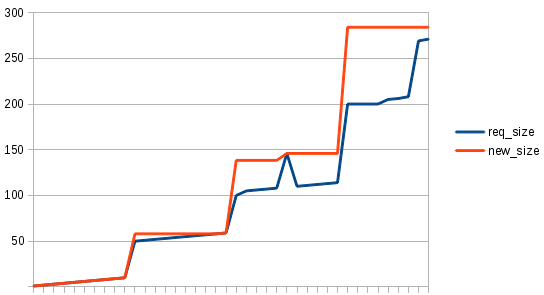
\includegraphics[width=10cm]{pics/realloc}
  \caption{New realloc method.}
  \label{figure:realloc}
\end{figure}

\input{mem/vralloc}
\chapter{Virtual Memory}

Each process owns their own master page table, in contrast to some kernels where
there might be only one master page table or one partial master page table,
and varying number of level two page tables. The kernel, also known as proc 0,
has its own master page table that is used when a process executes in kernel
mode, as well as when ever a kernel thread is executing. Static or fixed page
table entries are copied to all master page tables created. A process shares its
master page table with its childs on \verb+fork()+ while \verb+exec()+ will
trigger a creation of a new master page table.

Virtual memory is managed as virtual memory buffers (\verb+struct buf+) that
are suitable for in-kernel buffers, IO buffers as well as user space memory
mappings. Additionlly the buffer system supports copy-on-write as well as
allocator schemes where a part of the memory is stored on a secondary
storage (i.e. paging).

Due to the fact that \verb+buf+ structures are used in different allocators
there is no global knowledge of the actual state of a particular allocation,
instead each allocator should/may keep track of allocation structs if desired
so. Ideally the same struct can be reused when moving data from a secondary
storage allocator to vralloc memory (physical memory). However we
always know whether a buffer is currently in core or not (\verb+b_data+) and
we also know if a buffer can be swapped to a different allocator
(\verb+B_BUSY+ flag).

\section{Page Fault handling and VM Region virtualization}

\begin{enumerate}
\item DAB exception transfers execution to \verb+interrupt_dabt+ in \verb+XXX_int_handlers.S+
\item \verb+mmu_data_abort_handler()+ (\verb+XXX_mmu.c+) gets called
\item to be completed...
\end{enumerate}


  \part{Process and Thread Management}

\chapter{Processes and Threads}

The process and thread management in Zeke is based on an idea that a
process is a container for threads owned by the process and it manages the
memory space and resources used by its threads. Naturally this means that a
process must always own at least one thread, that is the main thread and all
other threads are children of the main thread. While a process is an unit
or a context of resource allocation, a thread is an object describing the
execution state, in other words a unit of execution, of an user space
application. Any process not having a main thread is immediately removed
from the system because there is nothing to execute.

Since a process is a container containing the main thread, and other threads,
there is no global execution state for a process, like in some other operating
systems. Some operating systems may use the main thread status as the process
state but Zeke makes an isolation between the process state and the thread
state. Thus a currently running process is mostlikely in \verb+READY+ state
for most of the time.

\section{A thread}

\subsection{The thread management concept}

\begin{figure}
  \center
  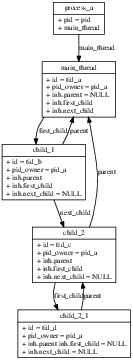
\includegraphics[width=7cm]{gfx/proc-classdiag}
  \caption{Thread tree example.}
  \label{figure:thtree}
\end{figure}

The following notation is used:

\begin{itemize}
  \item \verb+tid_X+ = Thread ID
  \item \verb+pid_a+ = Process ID
  \item \verb+0+ = NULL
\end{itemize}

\verb+process_a+ a has a main thread called \verb+main+. Thread
\verb+main+ has two child thread called \verb+child_1+ and \verb+child_2+.
\verb+child_2+ has created one child thread called \verb+child_2_1+.

\verb+main+ owns all the threads it has created and at the same time child
threads may own their own threads. If parent thread is killed then the
children of the parent are killed first in somewhat reverse order.

\begin{itemize}
  \item \verb+parent+ = Parent thread of the current thread if any
  \item \verb+first_child+ = First child created by the current thread
  \item \verb+next_child+ = Next child in chain of children created by the
        parent thread
\end{itemize}

\subsubsection{Examples}

\subparagraph*{process\_a is killed}

Before \verb+process_a+ can be killed \verb+main+ thread must be killed,
because it has child threads its children has to be resolved and killed in
reverse order of creation.

\subparagraph*{child\_2 is killed}

Killing of \verb+child_2+ causes \verb+child_2_1+ to be killed first.

\section{A process}

\begin{figure}
  \center
  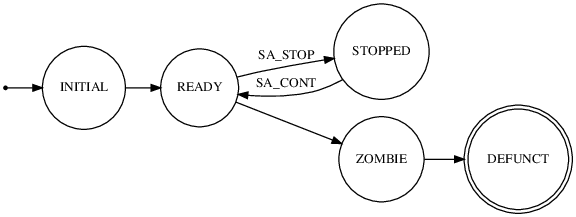
\includegraphics[width=10cm]{gfx/proc-states}
  \caption{Process states.}
  \label{figure:procstates}
\end{figure}

% TODO sections
Figure \ref{figure:procstates} shows all state transitions
of a process in Zeke.

Calling \verb+fork+ syscall causes a creation of a new process container,
cloning of the currently executing thread as a new main thread as well as
marking all current memory regions as copy-on-write regions for both processes.
Marking all currently mapped regions as COW makes it easy to get rid of
otherwise hard to solve race conditions.

When a process calls \verb+exec+ syscall the current main thread is replaced by
a newly created main thread that's pointing to the new process image, ie.
\acs{PC} is set to the entry point of the new image. Before \verb+exec+
transfers control to the new program the kernel will run resource cleanups and
inherit properties as mandated by the \acs{POSIX} standard.

\chapter{Scheduling}

\section{Thread scheduler}

The scheduler in Zeke is conceptually object oriented and all scheduling
entities, CPUs as well as scheduling policies are implemented as objects in the
scheduling system. Each CPU can be technically populated with a different set of
scheduling policies that are then only executable on that particular CPU, see
figure \ref{figure:objscheds}.

\begin{figure}
  \center
  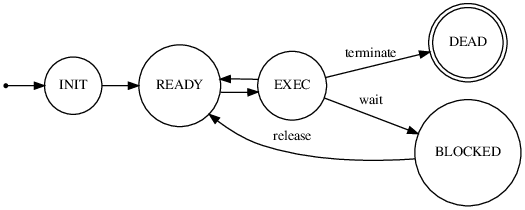
\includegraphics[width=10cm]{gfx/thread-states}
  \caption{Thread states in the scheduler.}
  \label{figure:threadstates}
\end{figure}

\begin{figure}
  \center
  \includegraphics[width=5cm]{proc/objscheds}
  \caption{Scheduler CPU objects for two processor cores and
           per scheduler object scheduling policy objects in
           priority order.}
  \label{figure:objscheds}
\end{figure}

\chapter{Executable File Formats}
\label{chap:exec}

\section{Introduction to executables in Zeke}

The kernel has a support for implementing loader functions for any new
executable format but currently only 32bit \acf{elf} support exist.
Loading of a new process image is invoked by calling exec syscall call that
calls \verb+load_image()+ function in \verb+kern/exec.c+ file.
Process image loaders are advertised by using \verb+EXEC_LOADER+ macro.

\section{ELF32}

The \acs{elf} loader in Zeke can be used to load statically linked executables
as well as anything linked dynamically. Currently only two loadable sections can
be loaded, code region and heap region.

\subsection{Suported \acs{elf} sections}

The kernel reads process memory regions based on information provided by
\verb+PT_LOAD+ sections in the \acs{elf} file.

The kernel can read additional information needed for executing a binary
from the elf notes. The non-standard notes are only parsed if \verb+Zeke+
is defined as an owner of the note.

\verb+NT_VERSION+

\verb+NT_STACKSIZE+

\verb+NT_STACKIZE+ note can be used to hint the kernel about the preferred
minimum size for the main thread stack.

\verb+NT_CAPABILITIES+

\verb+NT_CAPABILITIES+ note is used to inform the kernel about capabilities
required to execute a binary file. The elf loader attempts to set each
capability as an effective capability, which may fail if the capability
isn't in the bounding capabilities set. In case the file has
\ver+O_EXEC_ALTPCAP+ oflag set then the loader will first add the capabilities
found to the bounding capabilities set.

The user space implementation of these note types is discussed in section
\ref{sec:libc_elf}.

\chapter{Libc: Process and Thread Management}

\section{\acs{elf} support}\label{sec:libc_elf}

Zeke libc supports adding simple note sections to \acs{elf} files by using
macros provided by \verb+sys/elf_notes.h+ header file. As discussed
previously in chapter \ref{chap:exec}, some additional information about the
runtime environment requirements can be passed via note sections. For example,
a macro called \verb+ELFNOTE_STACKSIZE+ can be used for indicating the minimum
stack size needed by the main tread of an executable, see listing
\ref{list:hugestack}.

\lstinputlisting[label=list:hugestack,%
caption=hugestack.c]{../../usr/examples/hugestack.c}

\section{Pthread}
\subsection{Mutex}

\epigraph{Tis in my memory lock'd,\newline
          And you yourself shall keep the key of it.}{\textit{Hamlet}, 1, ii}



  \part{System Calls}

\chapter{Introduction to System Calls}

\section{Syscall flow sequence}

\begin{enumerate}
\item User scope thread makes a syscall by calling:
      \verb+syscall(SYSCALL_XXX_YYY, &args)+, where XXX is generally a
      module/compilation unit name, YYY is a function name and args is a
      syscall dataset structure in format declared in \verb+syscalldef.h+.

\item The interrupt handler calls \verb+_intSyscall_handler()+ function where
      syscall handler of the correct subsystem is resolved from
      \verb+syscall_callmap+.

\item Execution enters to the subsystem specific \verb+XXX_syscall()+
      function where the system call is either handled directly or a next level
      system call function is called according to minor number of
      the system call.

\item \verb+XXX_syscall()+ returns a \verb+uint32_t+ value which is, after
      multiple return steps, returned back to the caller which should know
      what type the returned value actually represents. In the future return
      value should be always integer value having the same size as register
      in the architecture. Everything else shall be passed both ways by using
      args structs, thus unifying the return value.
\end{enumerate}


\section{Syscall Major and Minor codes}

System calls are divided to major and minor codes so that major codes represents
a set of functions related to each other, usually all the syscall functions in a
single compilation unit. Major number sets are internally called groups. Both
numbers are defined in \verb+syscall.h+ file.


\chapter{Adding new syscalls and handlers}

\section{A new syscall}

\begin{itemize}
\item \verb+include/syscall.h+ contains syscall number definitions
\item \verb+include/syscalldef.h+ contains some useful structures that can be used when
      creating a new syscall
\item Add the new syscall under a syscall group handler
\end{itemize}

\section{A new syscall handler}

\begin{itemize}
\item Create a new syscall group into \verb+include/syscall.h+
\item Create syscall number definitions into the previous file
\item Add the new syscall group to the list of syscall groups in \verb+syscall.c+
\item Create a new syscall group handler
\end{itemize}


\chapter{sysctl}

The Zeke sysctl mechanism uses hierarchically organized \ac{MIB} tree as a
debugging and online configuration interface to the kernel. This is extremely
useful for example when testing scheduling parameters. Instead of recompiling
after every parameter change it is possible to change kernel's internal
parameters at run time by using sysctl interface.

There is only one syscall for sysctl which handles both reading/writing a
\ac{MIB} variable and queries to the MIB.

\section{Magic names}

There is some magic OID's that begins with \verb+{0,...}+ that are used for
queries and other special purposes. Particularly all OID's begin with 0 are
magic names. Currently allocated magic names are described in table
\ref{table:sysctlmagic}.

\begin{table}
\caption{sysctl magic names.}
\label{table:sysctlmagic}
\begin{tabular}{lll}
Name                & Internal function        & Purpose\\
\hline
\verb+{0,1,<iname>}+ & \verb+sysctl_sysctl_name()+     & Get the name of a MIB variable.\\
\verb+{0,2,<iname>}+ & \verb+sysctl_sysctl_next()+     & Get the next variable from MIB tree.\\
\verb+{0,3}+            & \verb+sysctl_sysctl_name2oid()+ & String name to integer name of the variable.\\
\verb+{0,4,<iname>}+ & \verb+sysctl_sysctl_oidfmt()+   & Get format and type of a MIB variable.\\
\verb+{0,5,<iname>}+ & \verb+sysctl_sysctl_oiddescr()+ & Get description string of a MIB variable.
\end{tabular}
\end{table}

\section{Adding new sysctl entries}

\subparagraph{Nodes}
New nodes containing sub-entries can be created with \verb+SYSCTL_NODE+ macro
like shown in listing \ref{list:sysctl_node}.

\lstinputlisting[label=list:sysctl_node,caption=Sysctl node macro.]{sys/sysctl_node.c}

In order to populate variables and nodes under newly created node the node
should be declared with \verb+SYSCTL_DECL(<name>);+, this can be done either in
\verb+sysctl.h+, in the header file of the subsystem/mode or locally in the
source code file. In the latter case the new node won't be available in
global scope.

\subparagraph{Variables}
\begin{itemize}
\item \verb+SYSCTL_STRING+
\item \verb+SYSCTL_INT+
\item \verb+SYSCTL_UINT+
\item \verb+SYSCTL_LONG+
\item \verb+SYSCTL_ULONG+
\item \verb+SYSCTL_COUNTER_U64+
\end{itemize}

\subparagraph{Procedures}
\lstinputlisting[label=list:sysctl_proc,caption=Adding a sysctl prodedure.]{sys/sysctl_proc.c}

\subparagraph{Feature test variables}
\verb+FEATURE(name, desc)+

  \input{ipc/ipc}
  \part{File System}

\chapter{File System Abstraction}

\section{General principles}

During this part of the document terms \acs{vnode} and \acs{inode} are
sometimes used interchangeably. Historically inode was a way to index files
in Unix-style file systems.\cite{Wikipedia:inode} While Zeke continues this
fashion it adds a concept of vnodes that are used as an abstraction level
between actual file systems and \acf{vfs}. This is done mostly in the same way
as on most of modern Unices today.

In Zeke vnodes are always used as a primary access method to the files in
a file system, inodes are only accessed internally within the file system
implementation code if the file system supports/uses inodes. Expected behavior
is that a vnode and a vnode number exist in the system as long as some process
owns a reference to that vnode. After there is no more references to a vnode
it's not guaranteed that the vnode exist in the memory and it cannot be
retrieved by using its vnode number. In fact normally vnodes can't be accessed
by their vnode number but a vnode number is guaranteed to be unique within
a single file system, superblock + vnode, but same vnode might be in use within
another file system and the number can be also reused.

To simplifify understanding how \acs{vfs} works in Zeke it can be described as
an object storage where file objects are first searched, found and the
associated (open) with a process. When a file is opened the process owns a
pointer to the file descriptor that contains some state information and pointer
to the actual file vnode. The vnode of the file is itself an object that knows
where contents of the file is stored (physical file system, superblock pointer)
and who knows how to manipulate the data (pointer to the vnode operations struct).
In fact vnode number itself is pretty much redundant and legacy information for
Zeke that is only provided for compatibility reasons, the actual access method
is always by a pointer reference to an object.

\section{Kernel interface}

Kernel interface to the actual file system drivers and file system superblocks
is built around virtual function structs defined in \acs{vfs} header file
\verb+fs.h+ and some user space header files defining unified data types.

A new file system is first registered to the kernel by passing a pointer to
fs struct that is a complete interface for mounting a new superblock and
interacting with the file system (note the difference between a file system
(driver) and a file system superblock that is referencing to the actual data
storage, while fs driver is accessing the superblock. The file system struct
is shown in \ref{list:fs}.

When superblock is mounted a superblock struct pointer is returned. This pointer
servers as the main interface to the newly mounted file system. Superblock is
defined as in listing \ref{list:fs_sb}. By using superblock function calls it's
possible to get direct references to vnodes and \acs{vnode} operations e.g. for
modifying file contents or adding new hard links to a directory node.

\lstinputlisting[label=list:fs,caption=fs struct definition.]{fs/fs.c}
\lstinputlisting[label=list:fs_sb,caption=superblock struct definition.]{fs/fs_superblock.c}

\section{VFS hash}

\verb+vfs_hash+ is an optional hashmap used for vnode caching for physically
slow file systems. VFS itself doesn't use this caching for any purpose so
it is completely optional to insert anything into there.

\chapter{fatfs}

\section{Overall description}

Fatfs driver is an implementation of \acf{fat} file system in Zeke.

\subparagraph{Main features}
\begin{itemize}
    \item \acs{fat}12/16/32,
    \item Supports multiple ANSI/OEM code pages including DBCS,
    \item \acf{lfn} support in ANSI/OEM or Unicode.
\end{itemize}

Note that Microsoft Corporation holds a patent for \ac{lfn} and commercial
use might be prohibitten or it may require a license form the company.
Therefore it's also possible to disable \acs{lfn} support in Zeke if required.

\chapter{procfs}

\section{Overall description}

Procfs is an implementation of a traditional process debugging interface in
Zeke. Procfs is a special file system containing entries for each process
in the system as well as some extra entries for runtime system information that
doesn't have any other obvious interface, like mounts file.

\subparagraph{System files}
\begin{itemize}
    \item mounts    - Showing all file system mounts in the system.
\end{itemize}

\subparagraph{Process specific files}
\begin{itemize}
    \item status    - Process status information.
    \item regions   - Contains information about memory regions mapped to
                      the process address space.
\end{itemize}

\chapter{ramfs}

\section{Overall description}

The purpose of the \acs{ramfs} is to provide a storage in RAM for temporary
files. This is important in user scope where there might be no other writable
storage medium available on some embedded platform. In addition to storage
for temporary files in user scope ramfs could be useful to store kernel files
as well, e.g. init can be unpacked from kernel to ramfs and then executed.

In the future ramfs code might be also useful for \acs{vfs} caching, so that
changes to a slow medium could be stored in ramfs-like structure and synced
later.

Ramfs should implement the same \acs{vfs} interface as any other regular
file system for Zeke. This ensures that the same POSIX compliant file
descriptor interface\footnote{POSIX file API is not actually yet implemented.}
can be used for files stored to ramfs as well as to any other file system.

\section{Structure of ramfs}

Data in Ramfs is organized by inodes, \acs{inode} can contain either a file or
directory entries, which means that an inode can be either files or directories.
Maximum size of a mounted ramfs is limited by size of \verb+size_t+ type.
Maximum size of a file is limited by size of \verb+off_t+ type. Figure
\ref{figure:inodes} shows a high level representation of how inodes are
organized and linked in ramfs to form directory tree with files and directories.

Contents of a file is stored in blocks of memory that are dynamically allocated
on demand. Block size is selected per file so all blocks are equal size and
block pointer array (\verb+in.data+) is expanded when new blocks are allocated
for a file. Figure \ref{figure:file} shows how memory is allocated for a file
inode.

Directory in ramfs is stored similarly to a file but \verb+in.dir+ (union with
\verb+in.data+) is now constant in size and it's used as a hash table which
points to chains of directory entries (directory entry arrays). If two files are
mapped to a same chain by hash function then the corresponding chain array is
re-sized so that the new entry can be added at the end of array. This means that
lookup from a directory entry chain is quite cache friendly and can usually
avoid fragmentation in memory allocation. Figure \ref{figure:dir} represents a
directory inode containing some directory entries.

\begin{figure}
  \center
  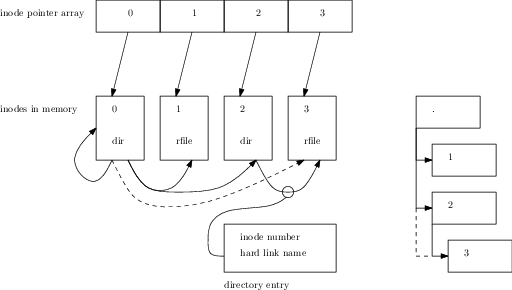
\includegraphics[width=15cm]{pics/inodes}
  \caption{Mounted ramfs with some inodes.}
  \label{figure:inodes}
\end{figure}

\begin{figure}
  \center
  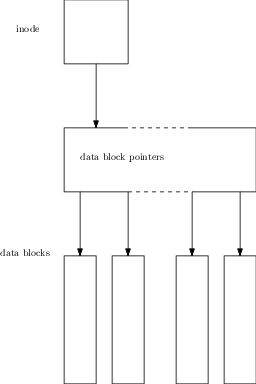
\includegraphics[width=7cm]{pics/file}
  \caption{Structure of a file stored in ramfs.}
  \label{figure:file}
\end{figure}

\begin{figure}
  \center
  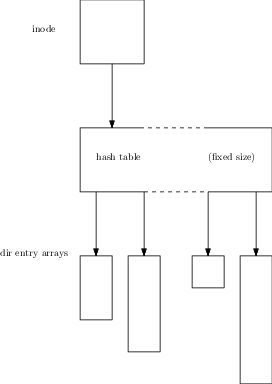
\includegraphics[width=7cm]{pics/dir}
  \caption{Directory containing some directory entries in ramfs.}
  \label{figure:dir}
\end{figure}


\section{Time complexity and performance analysis}

\subsection{Mount}

When a new ramfs superblock is mounted it's appended to the end of the global
superblock list. Time complexity of this operation is $O(n)$ as there is no
information about the last node in the list. However this is not a major
problem because new mounts happen relatively rarely and other operations during
the mounting process will take much more time than traversing a super block list
of any practical length. Those other operations includes allocating memory for
inode array, allocating memory for inode pool and initializing some data
structures etc.

\subsection{Get vnode by vnode number}

Index nodes are stored in contiguous array as shown in figure
\ref{figure:inodes}. This trivially means that a vnode can be always fetched
from mounted ramfs in $O(1)$ time as it's only a matter of array indexing.

\subsection{Lookup vnode by filename}

File lookup on ramfs level is implemented only on single directory vnode level
and sub-directory lookup must be then implemented on \acs{vfs} level i.e. lookup
function for a vnode can only lookup for entries in the current directory
vnode. A file lookup is made by calling \verb+vnode->vnode_ops->lookup()+.

Directory entries are stored in chained hash tables as shown in figure
\ref{figure:dir}. It can be easily seen that usually a chain array contains only
a single entry and therefore lookup is $O(1)$. In sense a of performance and
efficiency of a chain array with length greater than zero is more complex.
Trivially lookup from array is of course $O(n)$. What is interesting here is
how CPU caching works here. Even though directory entries are different in size
they are all stored in contiguous memory area and can be loaded to CPU cache
very efficiently, whereas many other data structures may lead to several
non-contiguous memory allocations that will pollute the caching and slow down
the lookup if there is only few entries. That said the current implementation of
directory entry storage seems almost perfect solution if amount of directory
entries is moderate and hash functions is good enough.\cite{Wikipedia:htable}

\subsection{Data by vnode}

Data stored in file inodes is accessed by calling
\verb+vnode->vnode_ops->read()+ and \verb+vnode->vnode_ops->write()+. Arguments
for both contains a pointer to the vnode, offset where to start reading or
writing from, byte count and a pointer to a buffer. Data structuring of a file
vnode was illustrated in figure \ref{figure:file}.

Pointer to a block of data by \verb+offset+ is calculated as shown in equation
\ref{eqn:dpointer}, where data is the data block pointer array. Length of
data pointer by the pointer is calculated as shown in equation \ref{eqn:dlen}.

\begin{eqnarray}
  \textrm{block} &=& \textrm{data} \left[ \frac{\textrm{offset} -
    (\textrm{offset} \& (\textrm{blksize} - 1))}{\textrm{blksize}}
    \right] \\
  \textrm{p}     &=& \textrm{block} \left[ \textrm{offset} \& (\textrm{blksize} - 1)
    \right] \label{eqn:dpointer} \\
  \textrm{len}  &=& \textrm{blocksize} - (\textrm{offset} \& (\textrm{blksize} - 1)) \label{eqn:dlen}
\end{eqnarray}

\subsection{Create a vnode}

Normally when a new inode is created it can be taken from the inode pool and
inserted at empty location on inode array. Average case can be considered to be
$O(1)$ then.

Lets consider a case where a new vnode is created and inserted to the index node
array but it's already full. A call to \verb+krealloc()+ will be issued and the
worst case of reallocation of a memory location may require to create a copy
of the whole index node array to a new location. This means that the worst case
time complexity of a vnode creation is relative to size of the array, so its
$O(n)$.

\subsection{Summary}

\begin{table}
  \caption{Summary of time complexity of ramfs functions.}
  \label{table:complexity}
  \begin{tabular}{lcc}
    Function & Average time complexity & Worst case time complexity \\
    \hline
    mount                 & $O(n)$ & $O(n)$ \\
    vnode by vnode number & $O(1)$ & $O(1)$ \\
    vnode by filename     & $O(1)$ & $O(n)$ \\
    data by vnode         & $O(1)$ & $O(1)$ \\
    create a new vnode    & $O(1)$ & $O(n)$
  \end{tabular}
\end{table}


\section{Performance testing}

Automated performance tests were implemented the same way as unit tests.
Ramfs performance tests are in \verb+test_ramfsperf.c+ file.

\subsection{Test results}

\subsection{Hard link operations}

Performance of hard link operations is tested in \verb+test_dehtableperf.c+.

Figure \ref{figure:dhlink_perf} shows performance measurements from
\verb+test_link_perf()+ test. In this test number of randomly named nodes are
added at every point and total time of adding those links is measured.
Name collisions are not handled but just appended to the chain array.
It seems that total time of \verb+dh_link()+ calls is almost flat but
it then starts to smoothly transform to something that is almost linearly
relative to the amount of links added. Calls to \verb+kmalloc()+ and
\verb+krealloc()+ seems to add some random behavior to link times.

Lookup tests were performed with \verb+test_lookup_perf()+ test and illustrated
in figure \ref{figure:dhlookup_perf}. The test works by first adding certain
amount of randomly named links and then trying to lookup with another set of
randomly selected names. Hit percentage is named as "\% found" in the plot and
lookup time is the mean of 100 random lookups. Lookup function seems to behave
quite linearly even though there is some quite strange deviation at some link
counts.

Even though lookups seems to be in almost linear relationship with the link
count of the directory entry hash table it doesn't mean lookups are slow.
Even with 20000 links average lookup takes only $45\:\mu s$ and it's very
rare to have that many directory entries in one directory.

\begin{figure}
  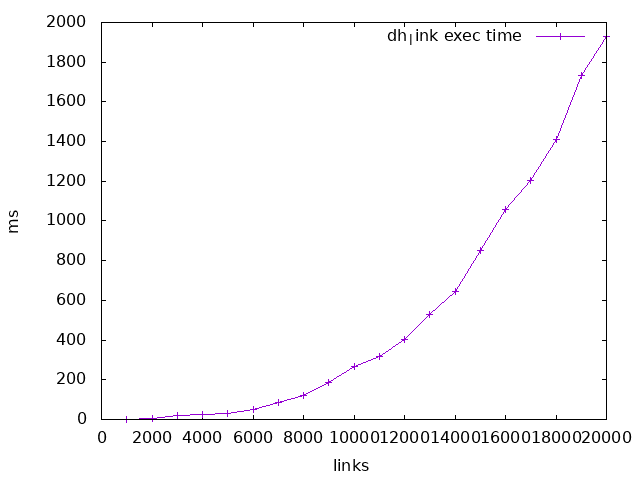
\includegraphics[width=15cm]{plots/dh_link}
  \centering
  \caption{Directory entry hash table link performance.}
  \label{figure:dhlink_perf}
\end{figure}

\begin{figure}
  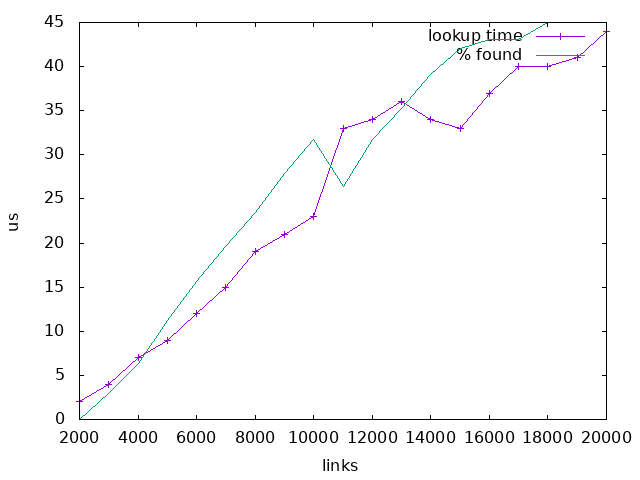
\includegraphics[width=15cm]{plots/dh_lookup}
  \centering
  \caption{Directory entry hash table lookup performance.}
  \label{figure:dhlookup_perf}
\end{figure}

\subsubsection{File operations}

Performance tests for file operations were performed on the universal target
where kmalloc uses malloc instead of dynem block allocator, this in fact may
make some of the result unreliable.

\begin{tabular}{l r@{.}l}
\textbf{Operation} &
\multicolumn{2}{c}{\textbf{Transfer speed (MB/s)}} \\
\hline
\textbf{Single write (100 MB)} && \\
new file      & 21&62 \\
existing file & 1694&92 \\
read          & 1098&90 \\
\textbf{Sequential writes} && \\
new file      & 9&06 \\
existing file & 335&80 \\
read          & 426&22 \\
\end{tabular}

\subsubsection{ramfs write/read performance}

Write and read performance testing is somewhat biased by the underlying kernel
even though we have our own memory allocator in place. Actually kmalloc may
make things work even worse because it's optimized for different kind of
suballocator that is not present on API level of Linux. So I think this is a
major cause for very poor memory allocation and first pass write performance
to the allocated blocks of memory, although kmalloc it self is quite inefficient
too.


\section{Suggestions for further development}

\subsection{Directories}

Directory entry lookup tables (hash tables) could be made variable in size.
This would make use of directory entry chains less frequent and greatly improve
performance of large directories while still maintaining small footprint for
small directories containing only few entries. At minimum this would only
require a function pointer to the current hash function in the inode. There is
no need to store the size of current hash table array in variable because it can
be determined by comparing the function pointer. So overhead of this improvement
would be size of \verb+size_t+ per directory and one more dereference per lookup.

\chapter{devfs}

\section{Overal description}

Devfs inherits ramfs and creates an abstraction layer between device drivers
and device driver abstraction layers. Essentially devfs creates a file
abstraction with vfs read() and write() functions that communicates with the
actual device driver.

\section{Device creation process}

Device registration with devfs starts from static init function of a subsystem,
device detection routine or some other triggering method. The device
identification/creation function shall, by some way, create a \verb+dev_info+
struct that describes the device and provides necessary function pointers for
reading and writing. Then \verb+make_dev(devXXX_info, 0, 0, 0666)+ is called
to register the device created. \verb+make_dev()+ then creates a fs node that is
contains a pointer to the provided \verb+dev_info+ in \verb+vn_specinfo+ of the
device.

There is some notable differences between devfs implementation of Zeke and other
common devfs or device abstractions in some other operating systems,
particularly Unices. First of all we don't use majorminor combination as a
device idetentifier, it's only provided for compatibility reasons and not used
for anything actually.\footnote{Some drivers may still use those internally but
there is no external interface provided. Uart is one of those using minor
numbers for internal indexing.} So devices can't be accessed by creating
a device file anywhere in the system, device files in Zeke are very special and
only ones that are created with \verb+make_dev()+ are valid, since the object
oriented model of Zeke VFS.

Another difference is that Zeke does not have character and block device
access modes/file types like most of traditional Unices. Zeke can support
buffered writes but it's always hidden from the user space. In practice,
it means that every user reading from a device file will always see the
same state, eg. if one process would write by using block device and another
one reading character device, the latter one would get either old data or
corrputed data. In fact there is no reason to have different file types for
different device types, block device files were designed to be a special file
type for hard disks, for some reason, but it doesn't make any sense to do it
that way in a modern kernel.\cite{Kamp:rethinkdev} Thus block device files are
not supported in Zeke and buffered access is not implemented but technically
supported inside the kernel.

\section{UART devices}

UART devices are handled by UART submodule (\verb+kern/hal/uart.c+) so that
common code between UART implementations can be shared and tty numbering can
be centrally organized. To register a new UART port the device driver has to
allocate a new \verb+uart_port+ structure and pass it to
\verb+uart_register_port()+ which finally registers the a new device file for
the port.

\begin{figure}
  \center
  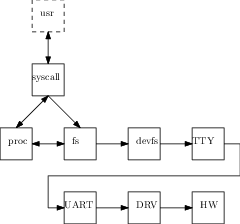
\includegraphics[width=9cm]{pics/uart}
  \caption{Communication between subsystems when a user process is writing to a UART.}
  \label{figure:fsuart}
\end{figure}



  \chapter{Libc: Process and Thread Management}

\section{\acs{elf} support}\label{sec:libc_elf}

Zeke libc supports adding simple note sections to \acs{elf} files by using
macros provided by \verb+sys/elf_notes.h+ header file. As discussed
previously in chapter \ref{chap:exec}, some additional information about the
runtime environment requirements can be passed via note sections. For example,
a macro called \verb+ELFNOTE_STACKSIZE+ can be used for indicating the minimum
stack size needed by the main tread of an executable, see listing
\ref{list:hugestack}.

\lstinputlisting[label=list:hugestack,%
caption=hugestack.c]{../../usr/examples/hugestack.c}

\section{Pthread}
\subsection{Mutex}

\epigraph{Tis in my memory lock'd,\newline
          And you yourself shall keep the key of it.}{\textit{Hamlet}, 1, ii}


  \input{test/test}

  \bibliography{zeke.bib}{}
  \bibliographystyle{plain}

\end{document}
